 \documentclass[xcolor=dvipsnames,table]{beamer}
%o
%e

\usepackage{latexsym}
\usepackage [ansinew]{inputenc}
\usepackage[brazil]{babel}
\usepackage{amssymb} %Este e o AMS paquete
\usepackage{amsmath}
\usepackage{stmaryrd}
\usepackage{fancybox}
\usepackage{datetime}
\usepackage{enumitem}

\usepackage[T1]{fontenc}

%\usepackage{beamerthemesplit}
\usepackage{graphicx}
\usepackage{graphics}
\usepackage{url}
\usepackage{algorithmic}
\usepackage{algorithm}
\usepackage{acronym}
\usepackage{array}

\newtheorem{definicao}{Definio}
\newcommand{\tab}{\hspace*{2em}}

\mode<presentation>
{
  %\definecolor{colortexto}{RGB}{153,100,0}
  \definecolor{colortexto}{RGB}{0,0,0}
  
% \setbeamersize{sidebar width left=0.5cm}
  \setbeamertemplate{background canvas}[vertical shading][ bottom=white!10,top=white!10]
%   \setbeamercolor{title}{fg=colortitulo!80!black,bg=blue!20!white}
%   \setbeamercolor{title}{bg=colortitulo!20!black}
%   \setbeamercolor{background canvas}{bg=colortitulo}
%   \setbeamercolor{frametitle}{fg=red}

  \setbeamercolor{normal text}{fg=colortexto} 

  \usetheme{Warsaw}
  %\logo{\includegraphics[width=2cm]{Images/ratonfuerte.jpg}}


%   \usefonttheme[onlysmall]{structurebold}
%   \usecolortheme{seahorse}
%  \usecolortheme[named={YellowOrange}]{structure}
%   \usecolortheme[named={Blue}]{structure}
%   \usecolortheme{crane}
%   \useoutertheme{default}
}

\title{Aut�mato Finito N�o-Determin�stico} 

\author{
  Esdras Lins Bispo Jr. \\ \url{bispojr@ufg.br}
}
 \institute{
  Linguagens Formais e Aut�matos \\Bacharelado em Ci�ncia da Computa��o}
\date{\textbf{12 de setembro de 2019} }

\logo{
\includegraphics[width=1cm]{images/ufjLogo.png}}

\begin{document}

	\begin{frame}
		\titlepage
	\end{frame}

	\AtBeginSection{
		\begin{frame}{Sum�rio}%[allowframebreaks]{Sum�rio}
    		\tableofcontents[currentsection]
    		%\tableofcontents[currentsection, hideothersubsections]
		\end{frame}
	}

	\begin{frame}{Plano de Aula}
		\tableofcontents
		%\tableofcontents[hideallsubsections]
	\end{frame}	
	
	\section{Instru��o pelos Colegas}
	
	\begin{frame}{Quest�o 032}	
		\begin{block}{[Q032]}
			Seja o AFN $M$, conforme o diagrama de estados abaixo. 
			\begin{center}
				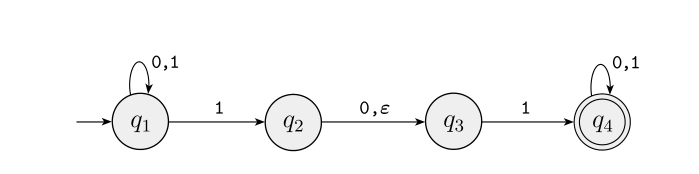
\includegraphics[width=.9\textwidth]{images/afn-n1}
			\end{center}
		Qual das cadeias abaixo \underline{n�o} � aceita por $M$?
		\end{block}
		\begin{enumerate}[label=(\Alph*)]
			\item {\sc 0110}
			\item {\sc 01011}
			\item {\sc 1001}
			\item {\sc 0101}
		\end{enumerate}
	\end{frame}

	\begin{frame}{Quest�o 033}	
		\begin{block}{[Q033]}
			Sobre o um AFN $M$, � \underline{incorreto} afirmar que...
		\end{block}
		\begin{enumerate}[label=(\Alph*)]
			\item para $M$ aceitar $\omega$, � necess�rio que todos os ramos de execu��o aceitem $\omega$.
			\item a sua fun��o $\delta$ tenha como sa�da um conjunto de estados.
			\item a sua fun��o de $\delta$ tem como uma de suas entradas um s�mbolo de $\Sigma_{\epsilon}$.
			\item $M$ tem apenas um estado inicial.
		\end{enumerate}
	\end{frame}

	\begin{frame}{Quest�o 034}	
		\begin{block}{[Q034]}
			\begin{columns}
				\begin{column}{0.05\textwidth}\end{column}
				\begin{column}{0.35\textwidth}
					Seja o AFD $M$, conforme o diagrama de estados ao lado. \\$M$ \underline{aceita} qual cadeia, das alternativas abaixo?
				\end{column}
				\begin{column}{0.55\textwidth}
					\begin{center}
						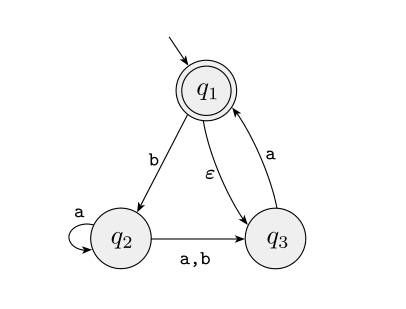
\includegraphics[width=0.8\textwidth]{images/afn-n4}
					\end{center}
				\end{column}
				\begin{column}{0.05\textwidth}\end{column}
			\end{columns}
		\end{block}
		\begin{enumerate}[label=(\Alph*)]
			\item {\sc bb}
			\item {\sc babba}
			\item {\sc b}
			\item {\sc ababa}
		\end{enumerate}
	\end{frame}
	
	\begin{frame}{Quest�o 035}	
		\begin{block}{[Q035]}
			Seja o AFN $M$, conforme o diagrama de estados abaixo. 
			\begin{center}
				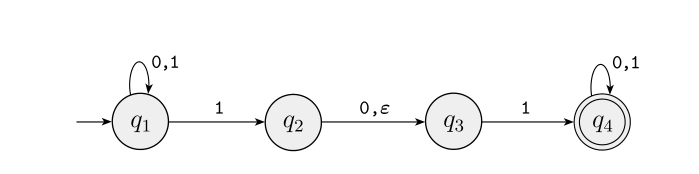
\includegraphics[width=.9\textwidth]{images/afn-n1}
			\end{center}
			Qual � o valor para $\delta(q_1,$ {\sc 1})?
		\end{block}
		\begin{enumerate}[label=(\Alph*)]
			\item $q_2$
			\item $\{q_1, q_2\}$
			\item $\emptyset$
			\item $\{q_1\}$
		\end{enumerate}
	\end{frame}

	\begin{frame}{Quest�o 036}	
		\begin{block}{[Q036]}
			Seja o AFN $M$, conforme o diagrama de estados abaixo. 
			\begin{center}
				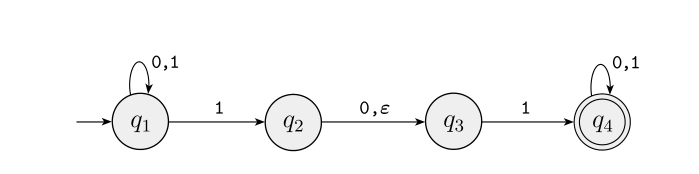
\includegraphics[width=.9\textwidth]{images/afn-n1}
			\end{center}
			Qual � o valor para $\delta(q_3,$ {\sc 0})?
		\end{block}
		\begin{enumerate}[label=(\Alph*)]
			\item $q_4$
			\item $\{q_3, q_4\}$
			\item $\emptyset$
			\item n�o pode ser definido.
		\end{enumerate}
	\end{frame}

	\begin{frame}{Quest�o 037}	
		\begin{block}{[Q037]}
			Na defini��o formal de computa��o para um AFN $N$, se $N$ aceita $\omega$, ent�o existe uma sequ�ncia de estados $r_0, r_1, \ldots, r_m$ em que
			\begin{itemize}
				\item - $r_0 = q_0$;
				\item - $\delta(r_i, \omega_{i+1}) \in r_{i+1}$, para $i=0, \ldots, m-1$, e
				\item - $r_m \in F$.
			\end{itemize}
			O que o valor de $m$ representa?
		\end{block}
		\begin{enumerate}[label=(\Alph*)]
			\item a quantidade de estados da sequ�ncia
			\item o tamanho da cadeia $\omega$
			\item a quantidade de entradas distintas de $\delta$
			\item a quantidade de estados de $N$
		\end{enumerate}
	\end{frame}

	
	\begin{frame}
		\titlepage
	\end{frame}
	
\end{document}